\begin{figure*}[t!]
\centering
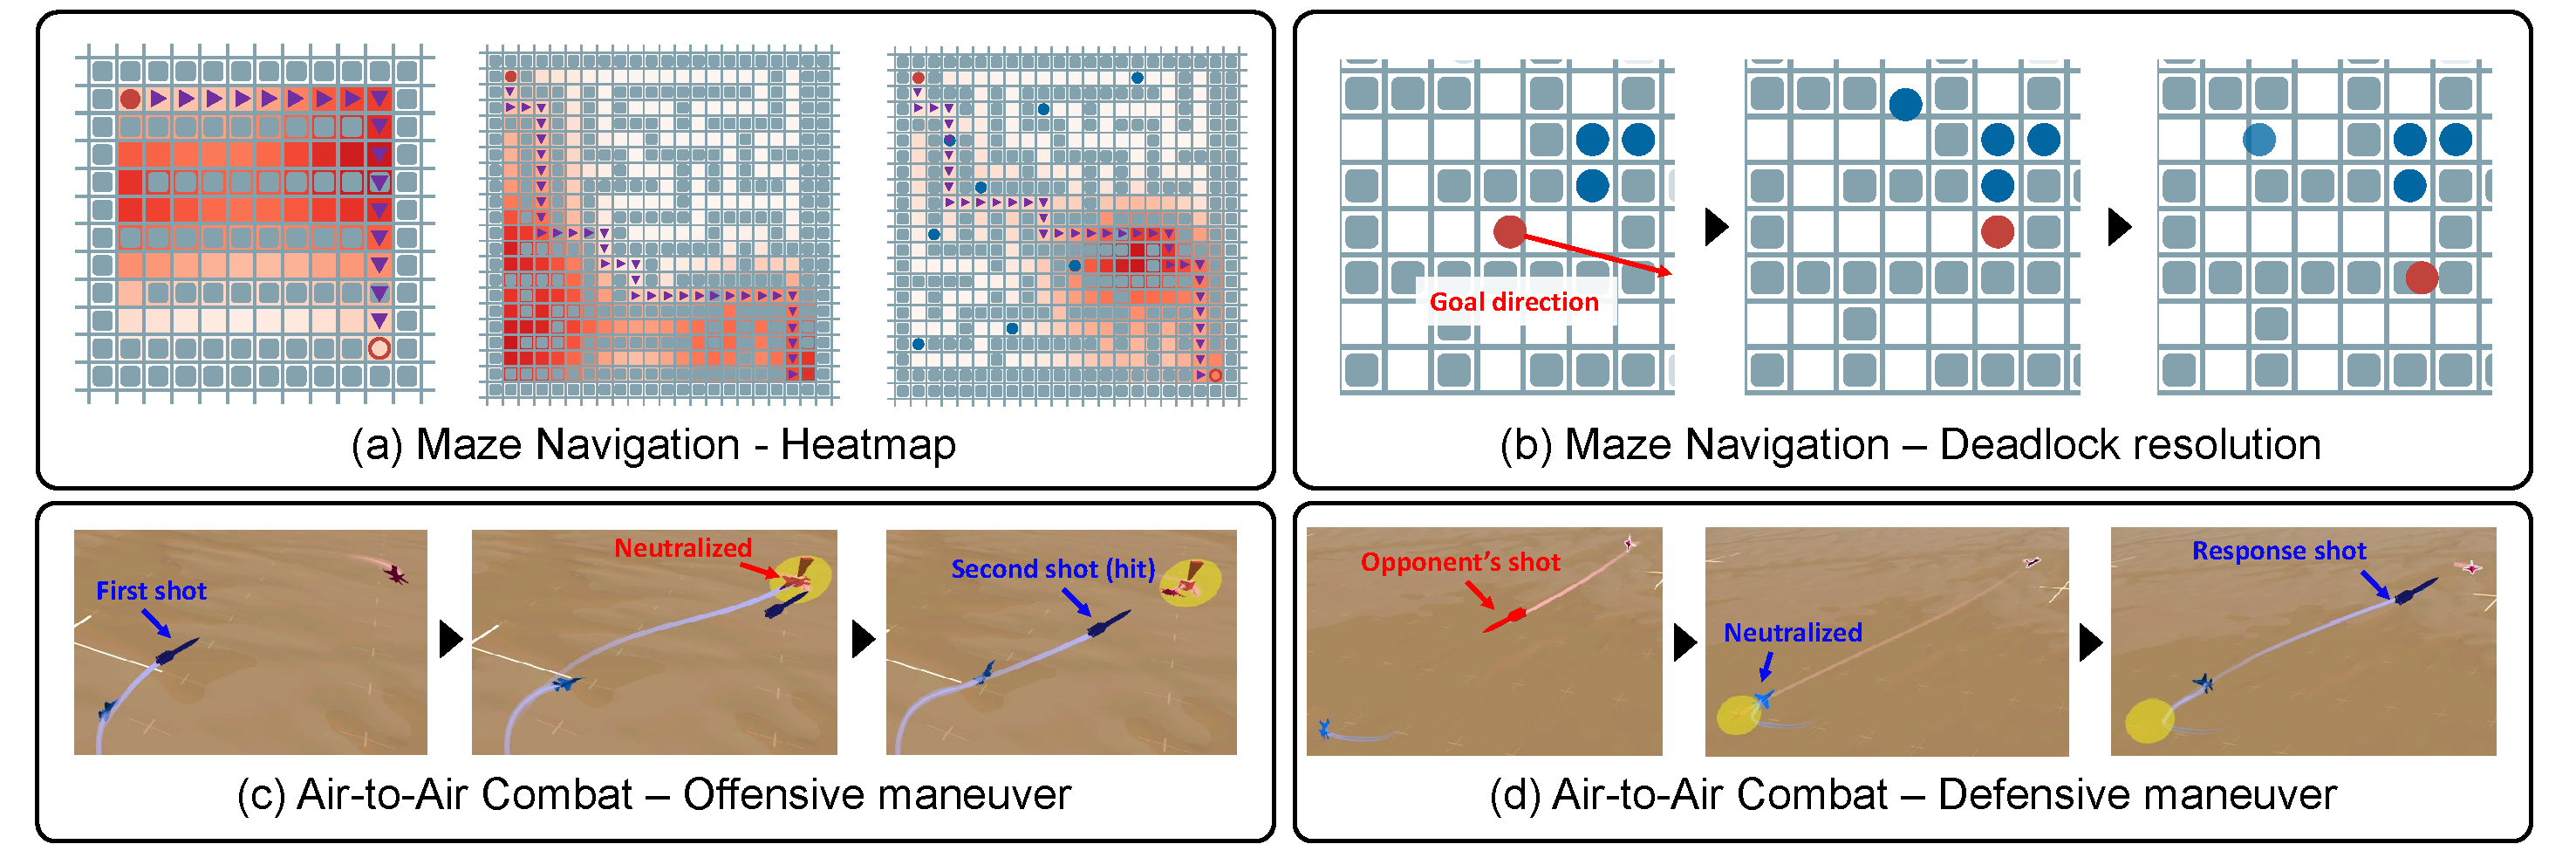
\includegraphics[width=\textwidth]{Figures/fig_5.pdf}
\caption{Representative qualitative results in (a)-(b) Maze Navigation and (c)-(d) Air-to-Air Combat. (a) Heatmaps in \emph{Easy}, \emph{Medium}, and \emph{Hard} scenarios, where the triangle marks the optimal path. Red indicates higher, while white indicates lower visitation frequency. (b) Deadlock examples, where the agent employs the \textsc{Penetration} action to navigate through cluttered corridors. (c) An offensive maneuver: the agent consecutively launches shots using the \textsc{Missile} action. (d) A defensive maneuver: the agent neutralizes the opponent's missile with a \textsc{Defense} action and responds with a counter shot.
\vspace{-10pt}
}
\label{fig:qual_result}
\end{figure*}

Table~\ref{tab:main_result} shows that TART outperforms the strongest PAMDP baseline in every scenario, with \emph{Success Rate} gains from $+2.7$ to $+13.2$ points.
Across all six scenarios, TART attains an average success rate of $87.2\%$, while the best baseline method (HyAR) achieves $77.4\%$.
Fig.~\ref{fig:quan_result} further shows that these gains do not come at the cost of resource efficiency.
In Maze Navigation, TART achieves lower or comparable \textbf{TTG}, indicating more efficient path completion.
In Air-to-Air Combat, TART also demonstrates efficiency in weapon usage by yielding lower or comparable \textbf{TTE} and \textbf{SPE}.
These results imply that TART leverages the fixed action budget more effectively with coordinated continuous maneuvers, as further evidenced by the qualitative analysis in Section V-C.

\subsubsection{Maze Navigation}
Since \textit{Easy} and \textit{Medium} do not contain dynamic obstacles, all methods yield \emph{Occupancy Coverage} near the shortest-path value.
The primary difference is efficiency, where TART demonstrates lower \textbf{TTG} and higher \emph{Success Rate}, while keeping \emph{Occupancy Coverage} near the shortest-path value.
In \textit{Hard}, background agents cause corridor congestion.
TART achieves lower \emph{Occupancy Coverage} and shorter \textbf{TTG}, which suggests that it unlocks bottlenecks with $\textsc{Penetration}$ rather than exploring widely.
The PAMDP actor-head baselines (PADDPG, PDQN, HPPO) and HyAR's cVAE approach do not couple discrete actions to subsequent maneuvers.
In contrast, TART learns a temporal representation and conditions the actor on a learned code.
This design triggers $\textsc{Penetration}$ precisely when it yields progress.
This behavior is consistent with the lower \emph{Occupancy Coverage} and shorter \textbf{TTG} observed on \textit{Hard}.

\subsubsection{Air-to-Air Combat}
Across all difficulty levels, TART achieves higher \emph{Success Rate} across all difficulties than baselines while maintaining \textbf{TTE} and \textbf{SPE} similar or lower.
This outcome is critical under limited-resource constraints.
Although deploying more missiles could raise success, the non-increasing \textbf{SPE} shows that TART achieves gains without higher consumption.
The reduced \textbf{SPE} observed in \textit{Easy} and \textit{Medium} reflects TART's ability to maintain lock-on after missile releases, resulting in more valid shots.
In \textit{Hard} scenario, success depends on effective use of the remaining $\textsc{Defense}$ actions against the armed opponent.
TART employs these actions more effectively through context-aware coordination of offensive and defensive maneuvers.
Overall, these findings show that temporal coupling between resource options (\emph{Missile, Defense}) and subsequent maneuvers enables efficient resource use and effective combat performance.